\section{Active Visual Exploration Based on Attention-Map Entropy}
\label{sec:ame}

\begin{figure}[th]
    \centering
    \begin{minipage}{0.6\linewidth}
        \centering
        \small\textit{A standard approach based on an auxiliary loss function}\\[3pt]
        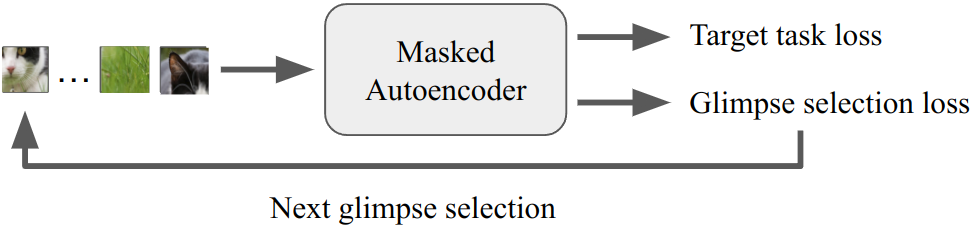
\includegraphics[width=\linewidth]{papers_src/AME/fig/teaser/1.png}
    \end{minipage}

    \vspace{10pt}

    \begin{minipage}{0.6\linewidth}
        \centering
        \small\textit{Our approach based on internal MAE uncertainty}\\[3pt]
        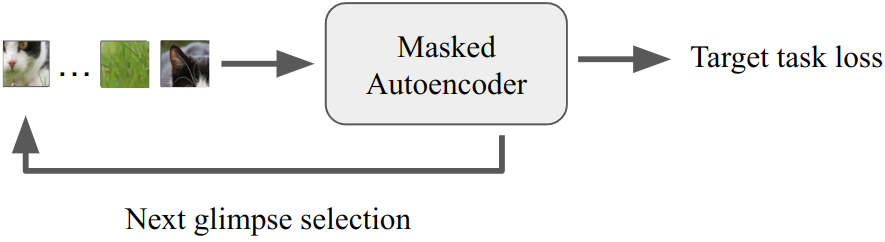
\includegraphics[width=\linewidth]{papers_src/AME/fig/teaser/2.png}
    \end{minipage}
    \caption[Attention-Map Entropy contrasted with auxiliary-loss glimpse selection]{\textbf{Attention-Map Entropy (AME).} The proposed approach chooses the most informative observations (patches) by reusing the internal uncertainty already coded in the attention maps of the target-task model. In contrast to existing methods, it does not require any auxiliary loss function dedicated to active exploration, so that training can concentrate entirely on the target-task loss. Figure reproduced~from~\pubcite{pardyl2023active}.}
    \label{fig:ame-teaser}
\end{figure}

\subsection{Motivation}
\label{sec:motivation-ame}

As established in Section~\ref{sec:uncertainty-scope}, prior work on glimpse-based active exploration relies on a dedicated network component, trained separately from and in parallel to the target task, to decide where to look next. This \emph{dual-objective} design has a tangible cost -- it increases the number of network components, raises the memory footprint, and complicates training, since two training objectives (one for the perceptual task, one for exploration) may pull in opposite directions.

This publication investigates Hypothesis~\ref{hyp:ame}: the uncertainty already encoded in a visual model's attention maps can be used to decide where to look next, without training a separate component for observation selection. A transformer-based masked autoencoder processing a partial view of a scene already produces a rich description of what it is uncertain about as the entropy of its self-attention maps. The question is if such a signal alone is sufficient to drive effective glimpse selection, and whether eliminating the second objective actually improves rather than harms performance (see Figure~\ref{fig:ame-teaser}).

\subsection{Attention-Map Entropy}

\begin{figure}[th]
    \centering
    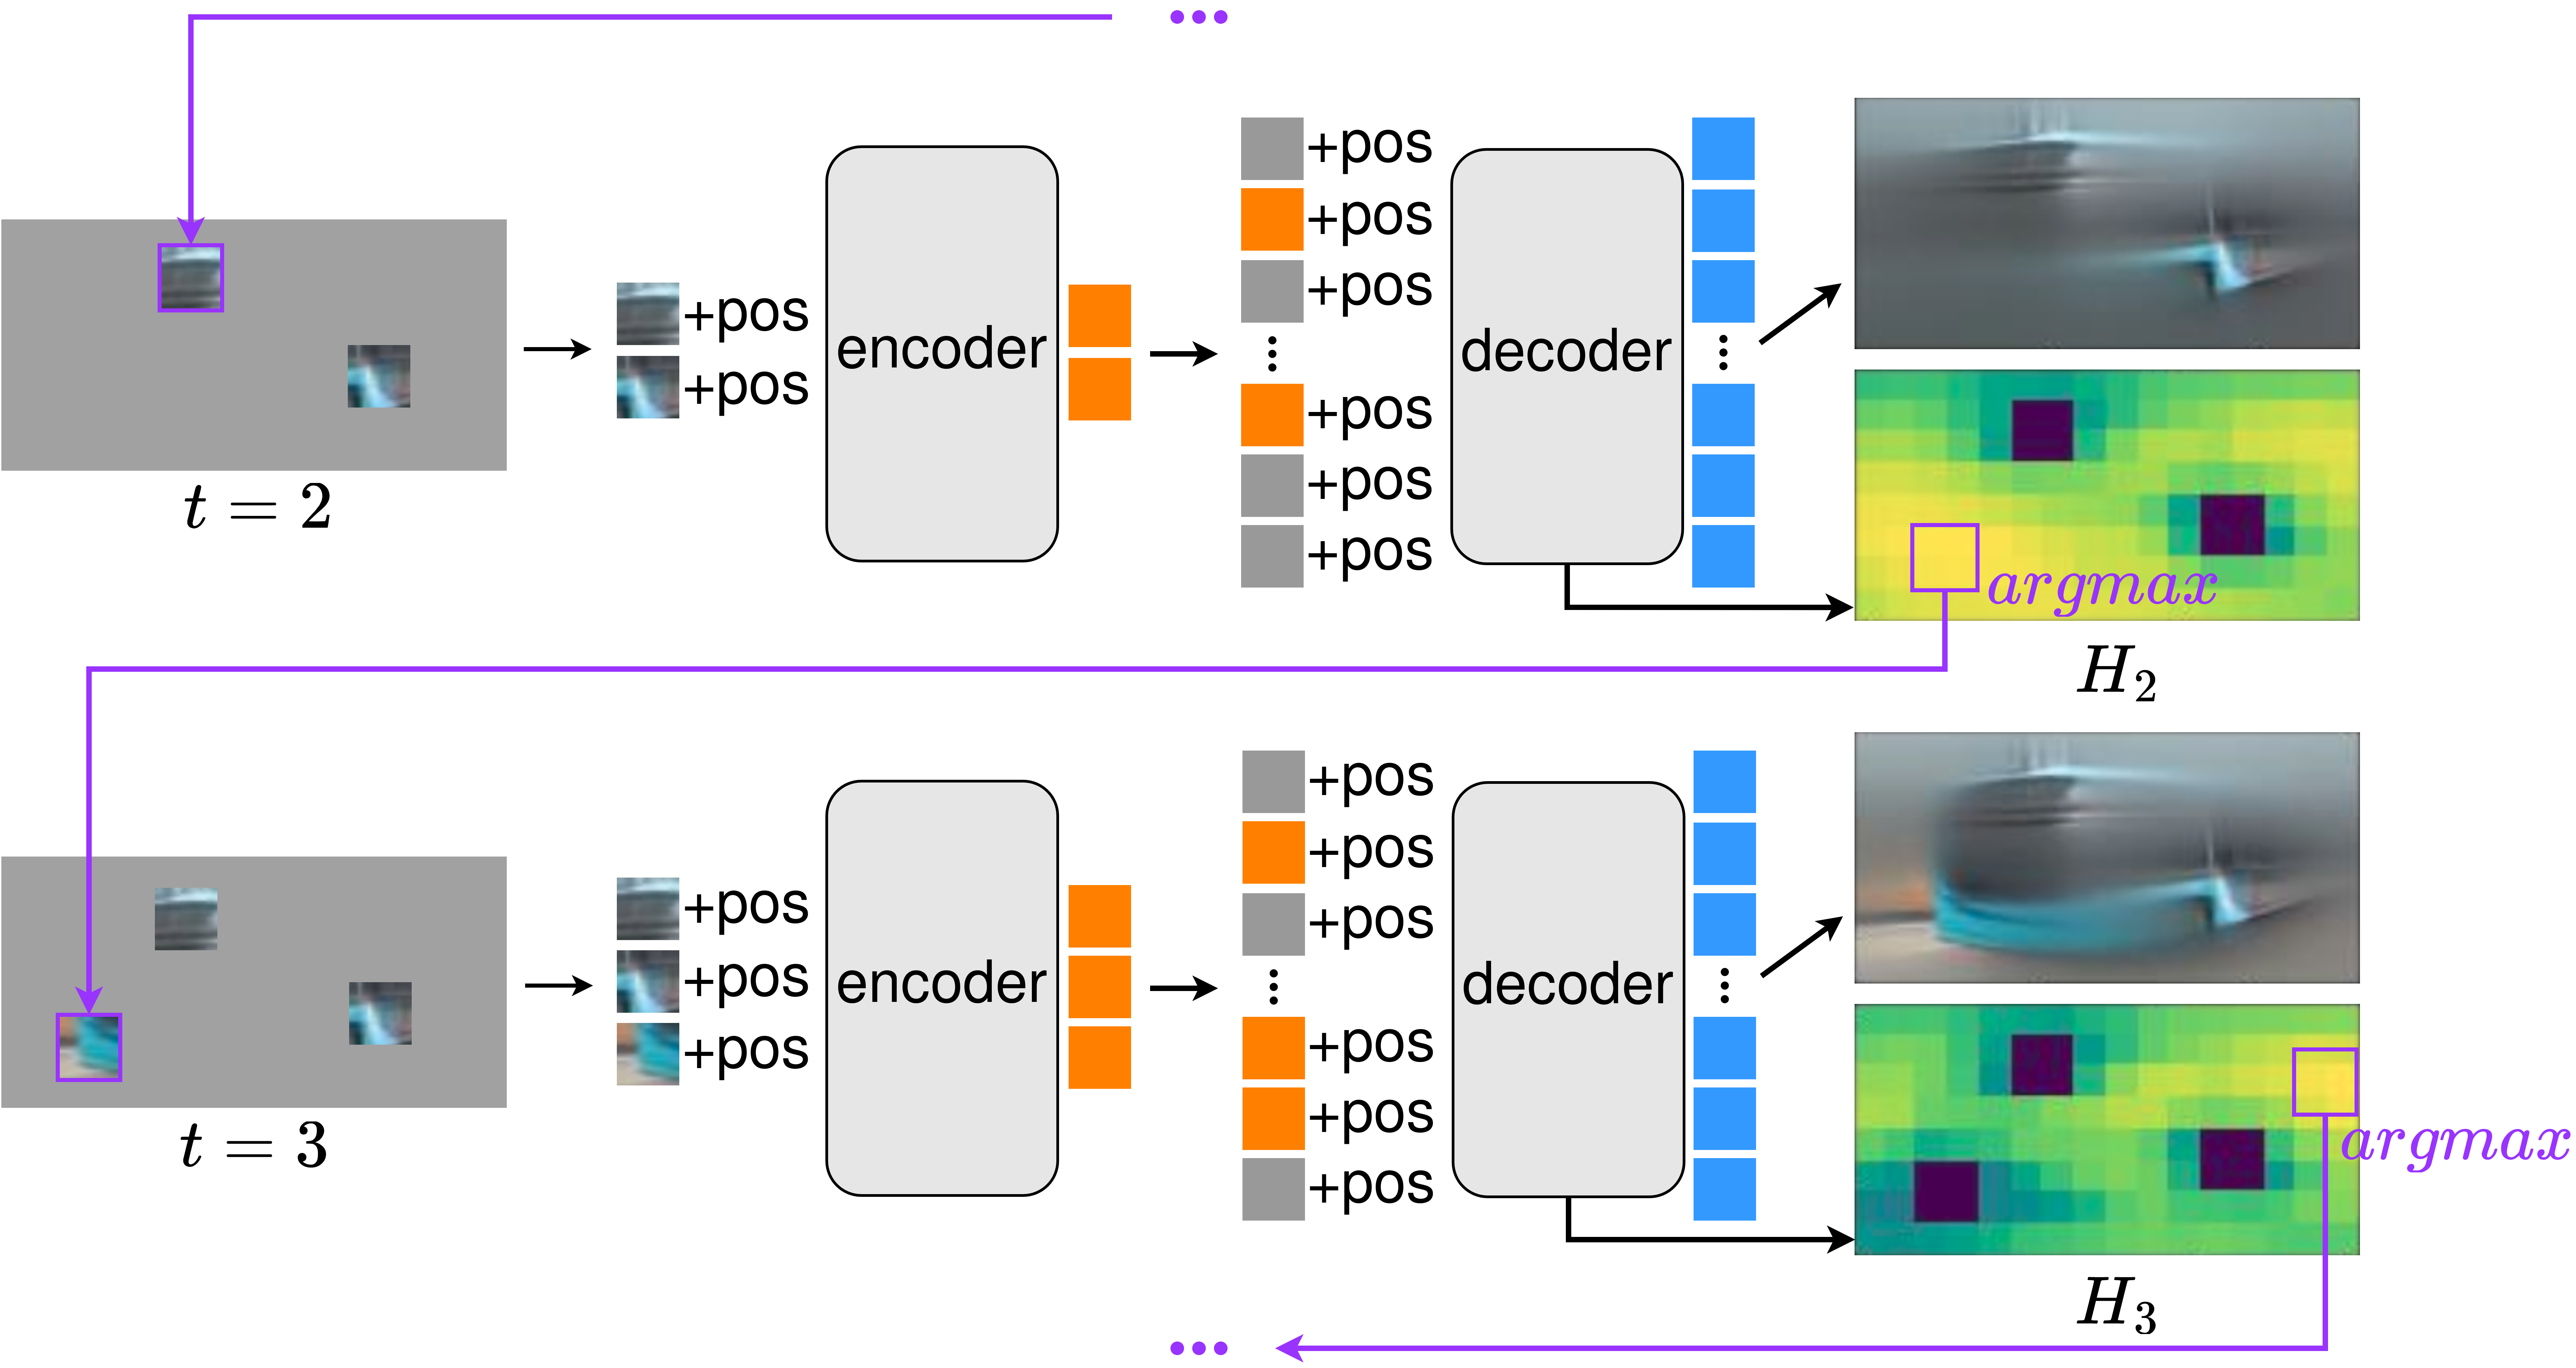
\includegraphics[width=\linewidth]{papers_src/AME/architecture.png}
    \caption[AME architecture for the reconstruction task]{\textbf{Architecture for reconstruction.} The agent has observed two patches of the image, which are processed by the encoder to produce their feature representations (orange rectangles). These outputs are combined with the masked patches (grey rectangles) and passed through the decoder, which reconstructs the missing image patches. In addition, the method computes the entropy map for one of the decoder's multi-head self-attention layers and uses it to select the location of the third glimpse (the one with the highest entropy). The process repeats until the assumed number of glimpses is reached. Reproduced~from~\pubcite{pardyl2023active}.}
    \label{fig:ame-architecture}
\end{figure}

\paragraph{Architecture.} The proposed method, named \emph{Attention-Map Entropy (AME)}, builds upon a masked autoencoder (Section~\ref{sec:prelim-vit-mae}) with a ViT-L encoder (24 transformer blocks and embedding size 1024) and a lightweight 8-block decoder (embedding size 512). At every step $t$, the encoder processes the $t$ glimpses observed so far, and the decoder combines their latent representations with mask tokens standing in for the unseen patches, producing an output for the target task. Figure~\ref{fig:ame-architecture} illustrates this process for the reconstruction task. For other tasks, the architecture is similar, with the exception of the output head.

\paragraph{Attention-derived uncertainty.} The key idea is to reuse the decoder's own self-attention maps to decide on the next action, instead of training a separate module for this purpose. Each row of a self-attention map is produced by a softmax and therefore defines a probability distribution describing how strongly the corresponding token attends to every other token when computing its representation. High entropy in a row indicates that the model cannot commit to any particular token as informative, which in turn signals that the underlying image region is poorly understood and would benefit from being observed. Because these distributions arise as a by-product of the target task's own forward pass, their entropy provides an uncertainty signal at no extra computational cost, with no additional parameters or training~objective~required.

For the single-patch glimpse regime, given the patches $p_1, \dots, p_t$ observed so far, the decoder operates on the full set of $M$ tokens, one for every patch position of the image grid: the $t$ observed patches plus mask tokens standing in for each position not yet observed. Each of its self-attention layers therefore computes an attention matrix
\begin{equation}
    A = \mathrm{softmax}\!\left(Q K^T / \sqrt{d_k}\right) \in \mathbb{R}^{M \times M},
    \label{eq:ame-attention}
\end{equation}
where $Q$ and $K$ pack together the query and key projections of all $M$ token embeddings produced by that layer, and $d_k$ is the dimension of the keys and queries. Row $i$ of $A$ is the probability distribution used to compute a weighted average of all patch representations when producing the updated representation of patch $i$. A peaked row means the model relies on a few already well-understood patches, while a flat row means it must combine evidence from many patches because none of them alone provides a confident answer. Figure~\ref{fig:ame-entropy} illustrates this on a toy $2\times2$ example.

\begin{figure}[th]
    \centering
    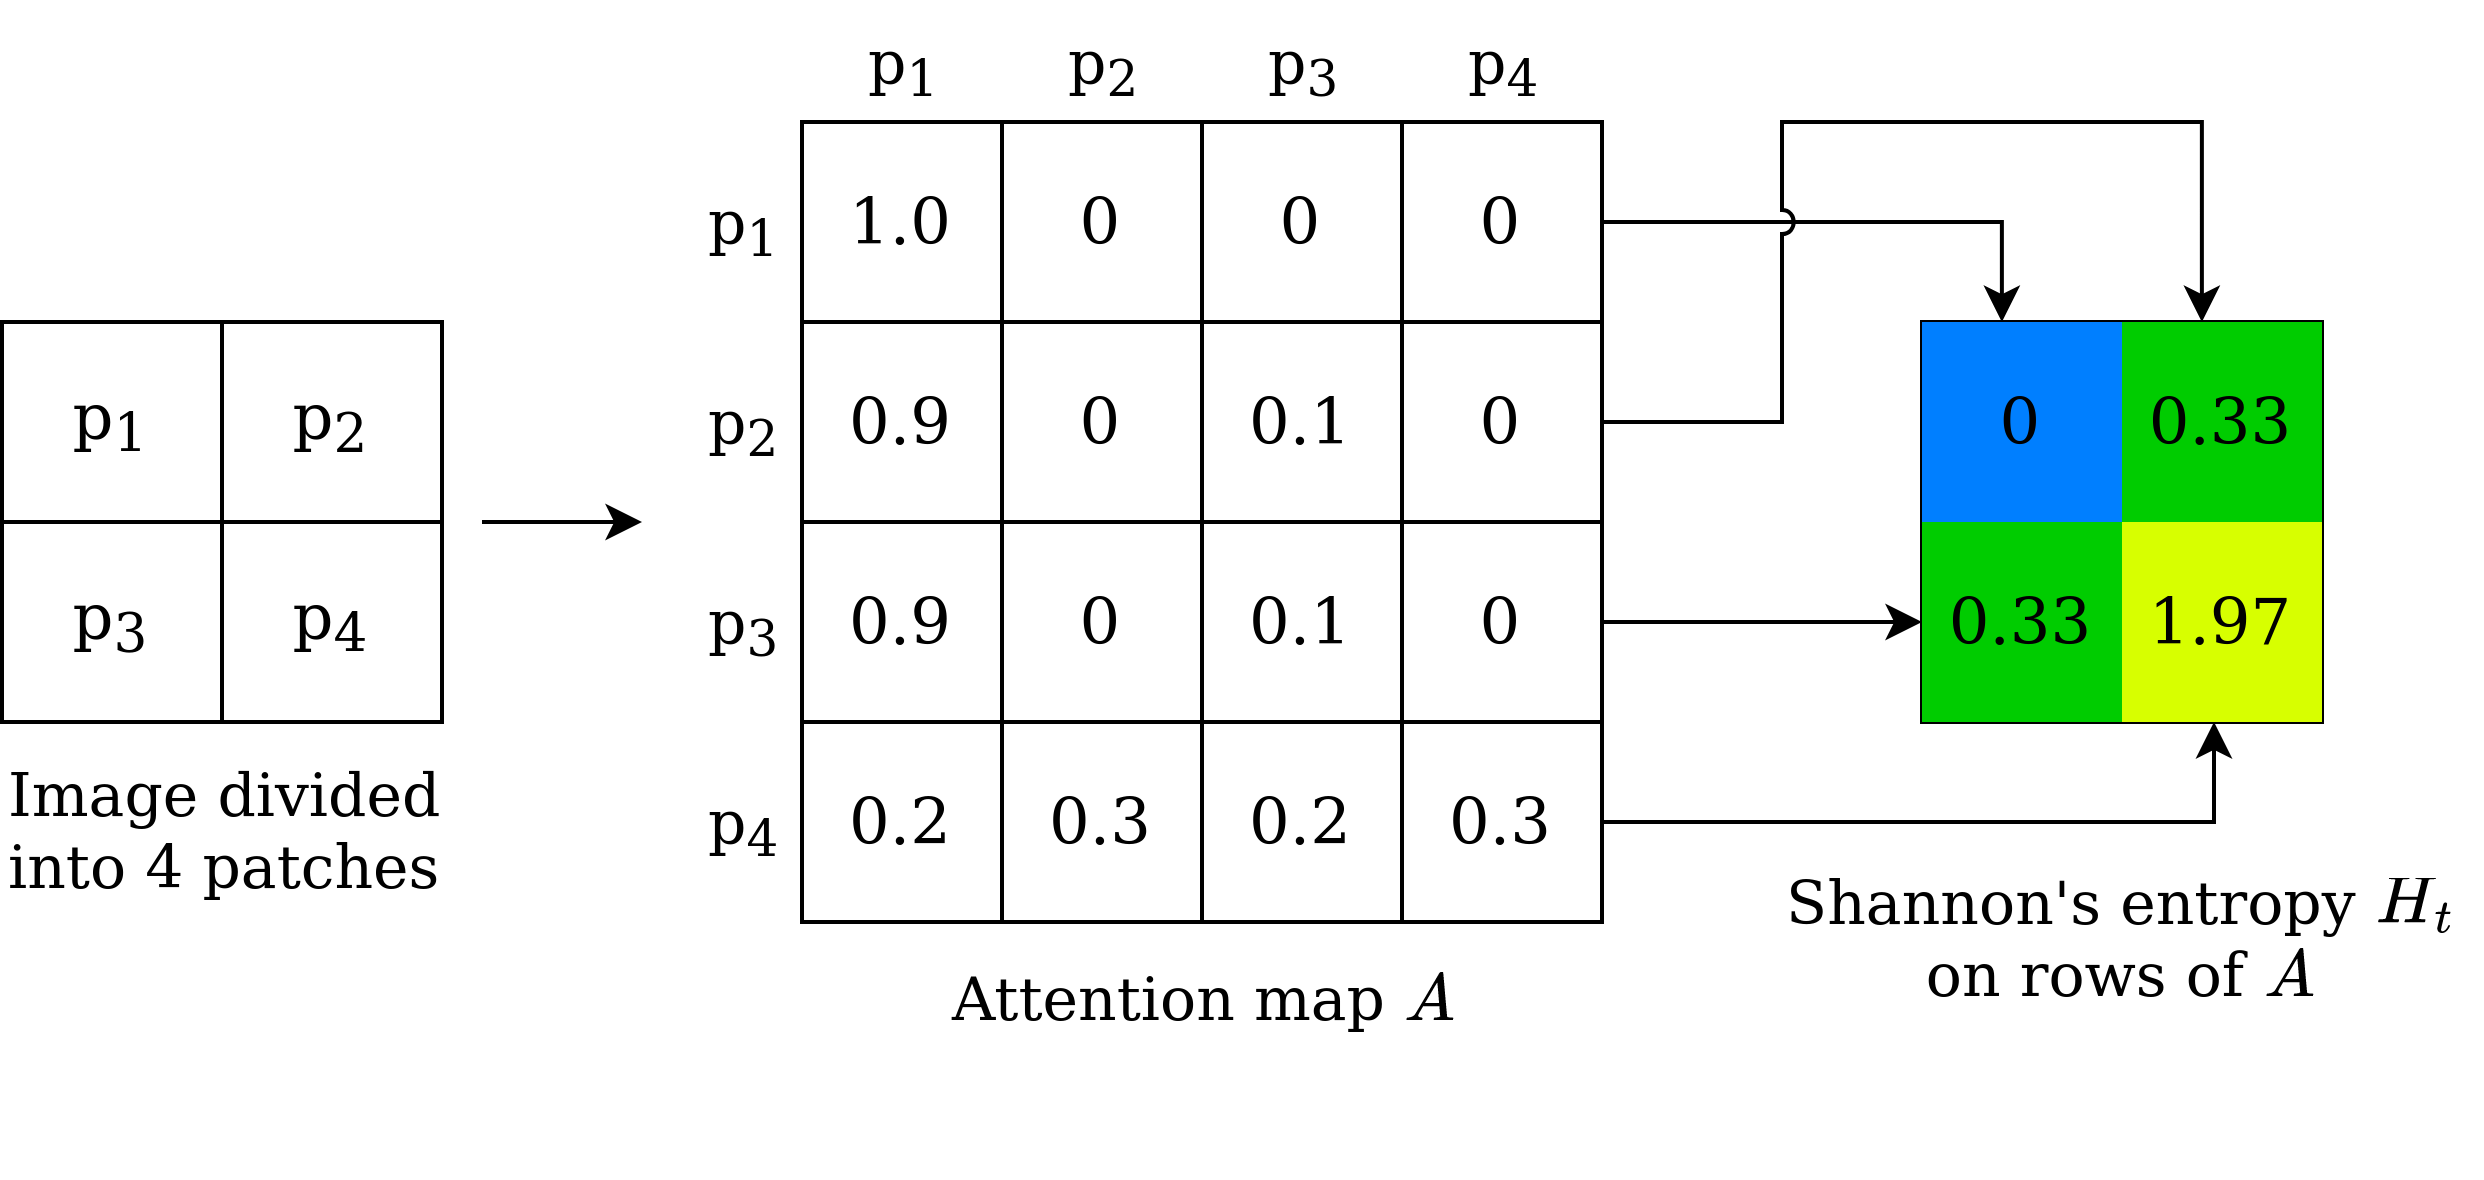
\includegraphics[width=0.75\linewidth]{papers_src/AME/fig/shannon.png}
    \caption[Illustration of an attention-derived entropy map]{\textbf{Entropy map.} Consider an image divided into four patches ($2\times2$), shown on the left. Its attention map is a $4\times4$ matrix, each row of which holds the attention weights used to compute the output of the corresponding patch in the next transformer layer. Computing the Shannon entropy (Equation~\ref{eq:shannon-entropy}) of each row yields a $2\times2$ entropy map; the patch with the highest entropy value is selected as the next glimpse. Figure reproduced~from~\pubcite{pardyl2023active}.}
    \label{fig:ame-entropy}
\end{figure}

\paragraph{Glimpse selection and task outputs.} Since transformers compute multiple attention maps in parallel (multi-head attention), the entropies contributed by all heads $h$ are summed into a single entropy map~at~step~$t$,
\begin{equation}
    H_t[i] = \sum_h H\!\left(A_{h,t}[i]\right),
    \label{eq:ame-entropy-map}
\end{equation}
where $A_{h,t}[i]$ is the $i$-th row of head $h$'s attention matrix at step $t$, and $H(\cdot)$ is the Shannon entropy of Equation~\ref{eq:shannon-entropy}. Entries corresponding to already-known patches are set to zero so that they are never re-selected, and the next glimpse is placed following a greedy selection strategy, i.e. at the position of maximal remaining entropy,
\begin{equation}
    i^* = \operatorname*{arg\,max}_i H_t[i].
    \label{eq:ame-argmax}
\end{equation}
For multi-patch glimpses, the entropy map is averaged over the glimpse footprint before selecting a location. The very first glimpse, for which no patch has yet been observed, is chosen by running the same procedure with only mask tokens as input. For reconstruction and segmentation, the decoder's final linear layer directly outputs pixel values or per-class logits for every patch. For classification, an auxiliary head attached to the encoder's \textsc{cls} token is trained jointly with the reconstruction objective. In every case, training uses only the losses of the perceptual tasks themselves, and no loss function or decision network dedicated to exploration is introduced.

\subsection{Experimental results}

The method is evaluated on three datasets: MS COCO~\cite{lin2014microsoft}, ADE20K~\cite{zhou2017scene}, and SUN360~\cite{xiao2012recognizing}, against two families of baselines, each tested under its corresponding glimpse regime: (i) $8 \times 48^2$ \emph{retinal} glimpses, matching the retina-like sensor simulation used by the convolutional methods AttSeg~\cite{seifi2020segment} and GlAtEx~\cite{seifi2021glimpse}, and (ii) $37\times16^2$ regular, non-retinal glimpses of a single ViT patch each, matching the transformer-based SimGlim~\cite{Jha2023WACV}.

\begin{table}[t]
    \caption[Reconstruction results across SUN360, ADE20K, and MS COCO]{\textbf{Reconstruction results:} Comparison of our model (AME) in the reconstruction task against AttSeg~\protect\cite{seifi2020segment}, GlAtEx~\protect\cite{seifi2021glimpse} and SimGlim~\protect\cite{Jha2023WACV} on SUN360, ADE20K and MS COCO datasets. The metric used is the root mean square error (RMSE; lower is better). For each experiment, we provide a training and evaluation regime defined by a number of glimpses of a specific resolution. Pixel \% and area \% denote respectively: the percentage of image pixels known to the model and the percentage of image area seen by the model. The two measures differ for retina-like glimpses, which have lower pixel densities in peripheral regions of the observation. Our method outperforms competing methods in~all~configurations.}
    \label{tab:ame-reconstruction}
    \begin{center}
    \begin{footnotesize}
    \begin{sc}
    \setlength{\tabcolsep}{4.5pt}
    \begin{tabular}{l@{\hspace{2pt}}rrrllrr}
    \toprule
    Method & SUN360 & ADE20K & MS COCO & Image res. & Glimpse regime & Pixel \% & Area \% \\
    \midrule
    AttSeg & 37.6 & 36.6 & 41.8 & $128 \times 256$ & $8 \times 48^2$ (retinal) & 18.75 & 56.25 \\
    GlAtEx & 33.8 & 41.9 & 40.3 & $128 \times 256$ & $8 \times 48^2$ (retinal) & 18.75 & 56.25 \\
    AME (ours) (retinal) & \textbf{23.6} & \textbf{23.8} & \textbf{25.2} & $128 \times 256$ & $8 \times 48^2$ (retinal) & 18.75 & 56.25\\
    \midrule
    AME (ours) (non-retinal) & 37.9 & 40.7 & 43.2 & $128 \times 256$ & $8 \times 16^2$ (non ret.) & 6.25 & 6.25\\
    AME (ours) (non-retinal) & 29.8 & 30.8 & 32.5 & $128 \times 256$ & $8 \times 32^2$ (non ret.) & 25.00 & 25.00\\
    AME (ours) (non-retinal) & \textbf{20.1} & \textbf{20.6} & \textbf{22.1} & $128 \times 256$ & $8 \times 48^2$ (non ret.) & 56.25 & 56.25 \\
    \midrule
    SimGlim (detached) & 26.2 & 27.2 & 29.8 & $224 \times 224$ & $37 \times 16^2$ (non ret.) & 18.75 & 18.75\\
    SimGlim (end-to-end) & 28.0 & 28.8 & 31.3 & $224 \times 224$ & $37 \times 16^2$ (non ret.) & 18.75 & 18.75 \\
    AME (ours) (non-retinal) & \textbf{23.4} & \textbf{26.2} & \textbf{28.6} & $224 \times 224$ & $37 \times 16^2$ (non ret.) & 18.75 & 18.75 \\
    \bottomrule
    \end{tabular}
    \end{sc}
    \end{footnotesize}
    \end{center}
\end{table}

\paragraph{Reconstruction.} As shown in Table~\ref{tab:ame-reconstruction}, AME achieves the best reconstruction RMSE across every dataset and glimpse regime tested, improving over both convolutional and transformer-based baselines. Non-retinal glimpses further improve scores over retinal ones by more than 10\%. The gain over SimGlim is particularly informative: since both methods share the same MAE backbone and differ only in the glimpse-selection rule, the improvement can be attributed to the entropy-based strategy itself rather than to the underlying architecture. Qualitative results on SUN360 in Figure~\ref{fig:ame-qualitative-retinal} confirm that the reconstructions produced by AME are visibly sharper and more detailed than those of the convolutional baselines.

\begin{figure}[t]
    \centering
    \newcommand{\qualimg}[1]{\includegraphics[width=2.8cm]{#1}}
    \begin{tabular}{c@{\hspace{3pt}}c@{\hspace{3pt}}c@{\hspace{3pt}}c}
        \toprule
        \small\textsc{Input} & \small\textsc{AME} (ours) & \small\textsc{GlAtEx} & \small\textsc{AttSeg} \\[3pt]
        \midrule
        \qualimg{papers_src/AME/fig/sun360/1/gt.jpg} &
        \qualimg{papers_src/AME/fig/sun360/1/ours.jpg} &
        \qualimg{papers_src/AME/fig/sun360/1/glatex.png} &
        \qualimg{papers_src/AME/fig/sun360/1/atseg.png} \\[2pt]
        \qualimg{papers_src/AME/fig/sun360/2/gt.jpg} &
        \qualimg{papers_src/AME/fig/sun360/2/ours.jpg} &
        \qualimg{papers_src/AME/fig/sun360/2/glatex.png} &
        \qualimg{papers_src/AME/fig/sun360/2/atseg.png} \\[2pt]
        \qualimg{papers_src/AME/fig/sun360/3/gt.jpg} &
        \qualimg{papers_src/AME/fig/sun360/3/ours.jpg} &
        \qualimg{papers_src/AME/fig/sun360/3/glatex.png} &
        \qualimg{papers_src/AME/fig/sun360/3/atseg.png} \\[2pt]
        \qualimg{papers_src/AME/fig/sun360/5/gt.jpg} &
        \qualimg{papers_src/AME/fig/sun360/5/ours.jpg} &
        \qualimg{papers_src/AME/fig/sun360/5/glatex.png} &
        \qualimg{papers_src/AME/fig/sun360/5/atseg.png} \\
        \bottomrule
    \end{tabular}
    \caption[Reconstruction quality comparison on SUN360]{\textbf{Reconstruction quality for SUN360.} Qualitative reconstruction results comparing AME against AttSeg~\cite{seifi2020segment} and GlAtEx~\cite{seifi2021glimpse} on the SUN360 dataset using $8\times48^2$ retinal glimpses. Reconstructions produced by our method are visibly sharper and better preserve scene structure. Reproduced~from~\pubcite{pardyl2023active}.}
    \label{fig:ame-qualitative-retinal}
\end{figure}

Figure~\ref{fig:ame-steps} visualises the process step by step: as additional glimpses are selected, the entropy map concentrates on the regions of the scene that remain blurry or unexplained, and the overall reconstruction, not only in the immediate neighbourhood of the newest glimpse, becomes progressively sharper.

\begin{figure}[!t]
    \centering
    % raised by half their height so the row labels sit vertically centred
    \newcommand{\amestepimg}[1]{\raisebox{-.5\height}{\includegraphics[width=2.5cm]{#1}}}
    \begin{tabular}{r c@{\hspace{1pt}}c@{\hspace{1pt}}c@{\hspace{1pt}}c c}
        \toprule
        Step & 1 & 3 & 5 & 8 & Ground truth \\
        \midrule
        Input &
            \amestepimg{papers_src/AME/fig/steps/1_masked.jpg} &
            \amestepimg{papers_src/AME/fig/steps/3_masked.jpg} &
            \amestepimg{papers_src/AME/fig/steps/5_masked.jpg} &
            \amestepimg{papers_src/AME/fig/steps/8_masked.jpg} & \\
        \addlinespace[1pt]
        Prediction &
            \amestepimg{papers_src/AME/fig/steps/1_out.jpg} &
            \amestepimg{papers_src/AME/fig/steps/3_out.jpg} &
            \amestepimg{papers_src/AME/fig/steps/5_out.jpg} &
            \amestepimg{papers_src/AME/fig/steps/8_out.jpg} &
            \amestepimg{papers_src/AME/fig/steps/0_input.jpg} \\
        \addlinespace[1pt]
        Entropy &
            \amestepimg{papers_src/AME/fig/steps/1_entropy.jpg} &
            \amestepimg{papers_src/AME/fig/steps/3_entropy.jpg} &
            \amestepimg{papers_src/AME/fig/steps/5_entropy.jpg} &
            -- & \\
        \bottomrule
    \end{tabular}
    \caption[Step-by-step AME glimpse selection on a sample scene]{\textbf{AME-based reconstruction step by step.} Selected steps of an $8\times32^2$ glimpse-selection process on a sample $256\times128$ image from ADE20K, showing the model input (known glimpses), its prediction, and the decoder attention entropy driving the choice of the next glimpse (known areas are explicitly set to zero). AME explores the image where its own reconstruction is still uncertain. Adapted~from~\pubcite{pardyl2023active}.}
    \label{fig:ame-steps}
\end{figure}

\paragraph{Classification.} Classification results on SUN360 are summarised in Table~\ref{tab:ame-classification}. AME achieves 75.7\% accuracy when training the full model end-to-end, compared to 56.4\% for GlAtEx, and 70.1\% when only the classification head is trained on top of frozen reconstruction features, still outperforming both convolutional baselines. The improvement in the head-only regime is particularly notable because the encoder was never exposed to any classification signal: the representations learned for reconstruction already provide a strong enough basis for scene-category decisions.

\begin{table}[t]
    \caption[Classification accuracy on SUN360]{\textbf{Classification results.} Multi-class classification accuracy on the SUN360 dataset using $8\times48^2$ retinal glimpses. \textit{Train-all} trains the entire model jointly; \textit{head-only} freezes the autoencoder weights and trains only the classification head on top. Our method (AME) outperforms competitive methods in both regimes. Reproduced~from~\pubcite{pardyl2023active}.}
    \label{tab:ame-classification}
    \centering
    \begin{footnotesize}
    \begin{sc}
    \begin{tabular}{lr}
        \toprule
        Method & Accuracy (\%) \\
        \midrule
        AttSeg & 52.6 \\
        GlAtEx (full) & 56.4 \\
        GlAtEx (no decoder) & 67.2 \\
        AME (ours) (head-only) & 70.1 \\
        AME (ours) (train-all) & \textbf{75.7} \\
        \bottomrule
    \end{tabular}
    \end{sc}
    \end{footnotesize}
\end{table}

\paragraph{Semantic segmentation.} Semantic segmentation on ADE20K follows the same pattern: AME raises pixel accuracy from 47.9\% (AttSeg) and 52.4\% (GlAtEx) to 70.3\%. The attached publication text reports~the~full~table.

\paragraph{Ablation studies.} Ablation studies confirm that the entropy-based rule is a reasonable heuristic, which is measurably better than naive alternatives. AME outperforms both uniformly random glimpse placement and a fixed, non-overlapping checkerboard pattern on both reconstruction and classification. A further ablation over which decoder layer the attention map is drawn from shows a consistent trend that entropy computed from deeper decoder layers, closer to the final output, yields better glimpse-selection decisions than entropy computed from shallow ones. See the attached publication text for more details.

\subsection{Contributions}
\label{sec:contributions-ame}

The publication summarised in this chapter makes the following contributions to visual exploration:

\begin{itemize}
    \item It introduces Attention-Map Entropy (AME), a glimpse-selection mechanism that reuses the entropy of a transformer decoder's own self-attention maps as a measure of the model's uncertainty about each unseen region. This removes the need for any auxiliary loss function or dedicated decision network for active exploration, in contrast to all prior approaches to this problem.
    \item It shows that a single, task-only training objective is sufficient to obtain a strong exploration policy, simplifying the training procedure compared to dual-objective designs.
    \item It provides, to the best of the authors' knowledge, the first published empirical evaluation coupling transformer-based active visual exploration with retina-like glimpses, mimicking a foveated sensor.
\end{itemize}

The task results and sampling-rule ablations confirm Hypothesis~\ref{hyp:ame} within the evaluated settings.

I was the first and primary author of this paper. I contributed to the conception of the idea and proposed using Shannon entropy as a measure of uncertainty, leading to the development of the AME method. I carried out the majority of the experimental design and implementation, conducted the majority of the experiments presented in the paper, and contributed significantly to writing the manuscript. I also presented the research at the International Joint Conference on Artificial Intelligence (IJCAI) 2023 in Macau. The code, data and further visualisations are available on my website at \url{https://io.pardyl.com/AME/}.
